% Copyright © 2013 Martin Ueding <dev@martin-ueding.de>

% Copyright © 2012-2013 Martin Ueding <dev@martin-ueding.de>

% This is my general purpose LaTeX header file for writing German documents.
% Ideally, you include this using a simple ``% Copyright © 2012-2013 Martin Ueding <dev@martin-ueding.de>

% This is my general purpose LaTeX header file for writing German documents.
% Ideally, you include this using a simple ``% Copyright © 2012-2013 Martin Ueding <dev@martin-ueding.de>

% This is my general purpose LaTeX header file for writing German documents.
% Ideally, you include this using a simple ``\input{header.tex}`` in your main
% document and start with ``\title`` and ``\begin{document}`` afterwards.

% If you need to add additional packages, I recommend not doing this in this
% file, but in your main document. That way, you can just drop in a new
% ``header.tex`` and get all the new commands without having to merge manually.

% Since this file encorporates a CC-BY-SA fragment, this whole files is
% licensed under the CC-BY-SA license.

\documentclass[11pt, ngerman, fleqn, DIV=15, headinclude, BCOR=2cm]{scrartcl}

\usepackage{graphicx}

% Environment to quote the problem. Currently, this is just a new name for the
% quote environment.
\newenvironment{problem}{\begin{quote}\textsf{\textbf{Aufgabenstellung:}}\quad}{\end{quote}}

\setkomafont{caption}{\sf}
\setkomafont{captionlabel}{\usekomafont{caption}}

%%%%%%%%%%%%%%%%%%%%%%%%%%%%%%%%%%%%%%%%%%%%%%%%%%%%%%%%%%%%%%%%%%%%%%%%%%%%%%%
%                                Locale, date                                 %
%%%%%%%%%%%%%%%%%%%%%%%%%%%%%%%%%%%%%%%%%%%%%%%%%%%%%%%%%%%%%%%%%%%%%%%%%%%%%%%

\usepackage{babel}
\usepackage[iso]{isodate}

%%%%%%%%%%%%%%%%%%%%%%%%%%%%%%%%%%%%%%%%%%%%%%%%%%%%%%%%%%%%%%%%%%%%%%%%%%%%%%%
%                          Margins and other spacing                          %
%%%%%%%%%%%%%%%%%%%%%%%%%%%%%%%%%%%%%%%%%%%%%%%%%%%%%%%%%%%%%%%%%%%%%%%%%%%%%%%

\usepackage[parfill]{parskip}
\usepackage{setspace}
\usepackage[activate]{microtype}

\setlength{\columnsep}{2cm}

%%%%%%%%%%%%%%%%%%%%%%%%%%%%%%%%%%%%%%%%%%%%%%%%%%%%%%%%%%%%%%%%%%%%%%%%%%%%%%%
%                                    Color                                    %
%%%%%%%%%%%%%%%%%%%%%%%%%%%%%%%%%%%%%%%%%%%%%%%%%%%%%%%%%%%%%%%%%%%%%%%%%%%%%%%

\usepackage[usenames, dvipsnames]{xcolor}

\colorlet{darkred}{red!70!black}
\colorlet{darkblue}{blue!70!black}
\colorlet{darkgreen}{green!40!black}

%%%%%%%%%%%%%%%%%%%%%%%%%%%%%%%%%%%%%%%%%%%%%%%%%%%%%%%%%%%%%%%%%%%%%%%%%%%%%%%
%                         Font and font like settings                         %
%%%%%%%%%%%%%%%%%%%%%%%%%%%%%%%%%%%%%%%%%%%%%%%%%%%%%%%%%%%%%%%%%%%%%%%%%%%%%%%

% This replaces all fonts with Bitstream Charter, Bitstream Vera Sans and
% Bitstream Vera Mono. Math will be rendered in Charter.
\usepackage[charter, greekuppercase=italicized]{mathdesign}
\usepackage{beramono}
\usepackage{berasans}

% Bold, sans-serif tensors. This fragment is taken from “egreg” from
% http://tex.stackexchange.com/a/82747/8945 and licensed under `CC-BY-SA
% <https://creativecommons.org/licenses/by-sa/3.0/>`_.
\usepackage{bm}
\DeclareMathAlphabet{\mathsfit}{\encodingdefault}{\sfdefault}{m}{sl}
\SetMathAlphabet{\mathsfit}{bold}{\encodingdefault}{\sfdefault}{bx}{sl}
\newcommand{\tens}[1]{\bm{\mathsfit{#1}}}

% Bold vectors.
\renewcommand{\vec}[1]{\boldsymbol{#1}}

%%%%%%%%%%%%%%%%%%%%%%%%%%%%%%%%%%%%%%%%%%%%%%%%%%%%%%%%%%%%%%%%%%%%%%%%%%%%%%%
%                               Input encoding                                %
%%%%%%%%%%%%%%%%%%%%%%%%%%%%%%%%%%%%%%%%%%%%%%%%%%%%%%%%%%%%%%%%%%%%%%%%%%%%%%%

\usepackage[T1]{fontenc}
\usepackage[utf8]{inputenc}

%%%%%%%%%%%%%%%%%%%%%%%%%%%%%%%%%%%%%%%%%%%%%%%%%%%%%%%%%%%%%%%%%%%%%%%%%%%%%%%
%                         Hyperrefs and PDF metadata                          %
%%%%%%%%%%%%%%%%%%%%%%%%%%%%%%%%%%%%%%%%%%%%%%%%%%%%%%%%%%%%%%%%%%%%%%%%%%%%%%%

\usepackage{hyperref}
\usepackage{lastpage}

% This sets the author in the properties of the PDF as well. If you want to
% change it, just override it with another ``\hypersetup`` call.
\hypersetup{
	breaklinks=false,
	citecolor=darkgreen,
	colorlinks=true,
	linkcolor=darkblue,
	menucolor=black,
	pdfauthor={Martin Ueding},
	urlcolor=darkblue,
}

%%%%%%%%%%%%%%%%%%%%%%%%%%%%%%%%%%%%%%%%%%%%%%%%%%%%%%%%%%%%%%%%%%%%%%%%%%%%%%%
%                               Math Operators                                %
%%%%%%%%%%%%%%%%%%%%%%%%%%%%%%%%%%%%%%%%%%%%%%%%%%%%%%%%%%%%%%%%%%%%%%%%%%%%%%%

% AMS environments like ``align`` and theorems like ``proof``.
\usepackage{amsmath}
\usepackage{amsthm}

% Common math constructs like partial derivatives.
\usepackage{commath}

% Physical units.
\usepackage[output-decimal-marker={,}]{siunitx}

% Since I use mathdesign with italic uppercase greek characters, the Ohm unit will be displayed with an italic Ω by default. Units have to be roman, so this forces it the right way.
\DeclareSIUnit{\ohm}{$\Omegaup$}
\DeclareSIUnit{\division}{DIV}
\DeclareSIUnit{\voltss}{$\mathrm{V_{SS}}$}

% Word like operators.
\DeclareMathOperator{\acosh}{arcosh}
\DeclareMathOperator{\arcosh}{arcosh}
\DeclareMathOperator{\arcsinh}{arsinh}
\DeclareMathOperator{\arsinh}{arsinh}
\DeclareMathOperator{\asinh}{arsinh}
\DeclareMathOperator{\card}{card}
\DeclareMathOperator{\csch}{cshs}
\DeclareMathOperator{\diam}{diam}
\DeclareMathOperator{\sech}{sech}
\renewcommand{\Im}{\mathop{{}\mathrm{Im}}\nolimits}
\renewcommand{\Re}{\mathop{{}\mathrm{Re}}\nolimits}

% Fourier transform.
\DeclareMathOperator{\fourier}{\ensuremath{\mathcal{F}}}

% Roman versions of “e” and “i” to serve as Euler's number and the imaginary
% constant.
\newcommand{\ee}{\eup}
\newcommand{\eup}{\mathrm e}
\newcommand{\ii}{\iup}
\newcommand{\iup}{\mathrm i}

% Symbols for the various mathematical fields (natural numbers, integers,
% rational numbers, real numbers, complex numbers).
\newcommand{\C}{\ensuremath{\mathbb C}}
\newcommand{\N}{\ensuremath{\mathbb N}}
\newcommand{\Q}{\ensuremath{\mathbb Q}}
\newcommand{\R}{\ensuremath{\mathbb R}}
\newcommand{\Z}{\ensuremath{\mathbb Z}}

% Shape like operators.
\DeclareMathOperator{\dalambert}{\Box}
\DeclareMathOperator{\laplace}{\bigtriangleup}
\newcommand{\curl}{\vnabla \times}
\newcommand{\divergence}[1]{\inner{\vnabla}{#1}}
\newcommand{\vnabla}{\vec \nabla}

\newcommand{\half}{\frac 12}

% Unit vector (German „Einheitsvektor“).
\newcommand{\ev}{\hat{\vec e}}

% Scientific notation for large numbers.
\newcommand{\e}[1]{\cdot 10^{#1}}

% Mathematician's notation for the inner (scalar, dot) product.
\newcommand{\bracket}[1]{\left\langle #1 \right\rangle}
\newcommand{\inner}[2]{\bracket{#1, #2}}

% Placeholders.
\newcommand{\emesswert}{\del{\messwert \pm \messwert}}
\newcommand{\fehlt}{\textcolor{darkred}{Hier fehlen noch Inhalte.}}
\newcommand{\messwert}{\textcolor{blue}{\square}}
\newcommand{\punkte}{\phantom{xxxxx}}
\newcommand{\punktevon}[1]{\begin{flushright}/ #1\end{flushright}}

% Separator for equations on a single line.
\newcommand{\eqnsep}{,\quad}

% Quantum Mechanics
\usepackage{braket}

%%%%%%%%%%%%%%%%%%%%%%%%%%%%%%%%%%%%%%%%%%%%%%%%%%%%%%%%%%%%%%%%%%%%%%%%%%%%%%%
%                                  Headings                                   %
%%%%%%%%%%%%%%%%%%%%%%%%%%%%%%%%%%%%%%%%%%%%%%%%%%%%%%%%%%%%%%%%%%%%%%%%%%%%%%%

% This will set fancy headings to the top of the page. The page number will be
% accompanied by the total number of pages. That way, you will know if any page
% is missing.
%
% If you do not want this for your document, you can just use
% ``\pagestyle{plain}``.

\usepackage{scrpage2}

\pagestyle{scrheadings}
\automark{section}
\cfoot{\footnotesize{Seite \thepage\ / \pageref{LastPage}}}
\chead{}
\ihead{}
\ohead{\rightmark}
\setheadsepline{.4pt}

%%%%%%%%%%%%%%%%%%%%%%%%%%%%%%%%%%%%%%%%%%%%%%%%%%%%%%%%%%%%%%%%%%%%%%%%%%%%%%%
%                            Bibliography (BibTeX)                            %
%%%%%%%%%%%%%%%%%%%%%%%%%%%%%%%%%%%%%%%%%%%%%%%%%%%%%%%%%%%%%%%%%%%%%%%%%%%%%%%

\newcommand{\bibliographyfile}{../../zentrale_BibTeX/Central}
\bibliographystyle{apalike2}

%%%%%%%%%%%%%%%%%%%%%%%%%%%%%%%%%%%%%%%%%%%%%%%%%%%%%%%%%%%%%%%%%%%%%%%%%%%%%%%
%                                Abbreviations                                %
%%%%%%%%%%%%%%%%%%%%%%%%%%%%%%%%%%%%%%%%%%%%%%%%%%%%%%%%%%%%%%%%%%%%%%%%%%%%%%%

\newcommand{\dhabk}{\mbox{d.\,h.}}

%%%%%%%%%%%%%%%%%%%%%%%%%%%%%%%%%%%%%%%%%%%%%%%%%%%%%%%%%%%%%%%%%%%%%%%%%%%%%%%
%                                  Licences                                   %
%%%%%%%%%%%%%%%%%%%%%%%%%%%%%%%%%%%%%%%%%%%%%%%%%%%%%%%%%%%%%%%%%%%%%%%%%%%%%%%

\usepackage{ccicons}

\newcommand{\ccbysadetext}{%
	\begin{small}
		Dieses Werk bzw. Inhalt steht unter einer
		\href{http://creativecommons.org/licenses/by-sa/3.0/deed.de}{%
			Creative Commons Namensnennung - Weitergabe unter gleichen
		Bedingungen 3.0 Unported Lizenz}.
	\end{small}
}

\newcommand{\ccbysadetitle}{%
	Lizenz: \href{http://creativecommons.org/licenses/by-sa/3.0/deed.de}
	{CC-BY-SA 3.0 \ccbysa}
}
`` in your main
% document and start with ``\title`` and ``\begin{document}`` afterwards.

% If you need to add additional packages, I recommend not doing this in this
% file, but in your main document. That way, you can just drop in a new
% ``header.tex`` and get all the new commands without having to merge manually.

% Since this file encorporates a CC-BY-SA fragment, this whole files is
% licensed under the CC-BY-SA license.

\documentclass[11pt, ngerman, fleqn, DIV=15, headinclude, BCOR=2cm]{scrartcl}

\usepackage{graphicx}

% Environment to quote the problem. Currently, this is just a new name for the
% quote environment.
\newenvironment{problem}{\begin{quote}\textsf{\textbf{Aufgabenstellung:}}\quad}{\end{quote}}

\setkomafont{caption}{\sf}
\setkomafont{captionlabel}{\usekomafont{caption}}

%%%%%%%%%%%%%%%%%%%%%%%%%%%%%%%%%%%%%%%%%%%%%%%%%%%%%%%%%%%%%%%%%%%%%%%%%%%%%%%
%                                Locale, date                                 %
%%%%%%%%%%%%%%%%%%%%%%%%%%%%%%%%%%%%%%%%%%%%%%%%%%%%%%%%%%%%%%%%%%%%%%%%%%%%%%%

\usepackage{babel}
\usepackage[iso]{isodate}

%%%%%%%%%%%%%%%%%%%%%%%%%%%%%%%%%%%%%%%%%%%%%%%%%%%%%%%%%%%%%%%%%%%%%%%%%%%%%%%
%                          Margins and other spacing                          %
%%%%%%%%%%%%%%%%%%%%%%%%%%%%%%%%%%%%%%%%%%%%%%%%%%%%%%%%%%%%%%%%%%%%%%%%%%%%%%%

\usepackage[parfill]{parskip}
\usepackage{setspace}
\usepackage[activate]{microtype}

\setlength{\columnsep}{2cm}

%%%%%%%%%%%%%%%%%%%%%%%%%%%%%%%%%%%%%%%%%%%%%%%%%%%%%%%%%%%%%%%%%%%%%%%%%%%%%%%
%                                    Color                                    %
%%%%%%%%%%%%%%%%%%%%%%%%%%%%%%%%%%%%%%%%%%%%%%%%%%%%%%%%%%%%%%%%%%%%%%%%%%%%%%%

\usepackage[usenames, dvipsnames]{xcolor}

\colorlet{darkred}{red!70!black}
\colorlet{darkblue}{blue!70!black}
\colorlet{darkgreen}{green!40!black}

%%%%%%%%%%%%%%%%%%%%%%%%%%%%%%%%%%%%%%%%%%%%%%%%%%%%%%%%%%%%%%%%%%%%%%%%%%%%%%%
%                         Font and font like settings                         %
%%%%%%%%%%%%%%%%%%%%%%%%%%%%%%%%%%%%%%%%%%%%%%%%%%%%%%%%%%%%%%%%%%%%%%%%%%%%%%%

% This replaces all fonts with Bitstream Charter, Bitstream Vera Sans and
% Bitstream Vera Mono. Math will be rendered in Charter.
\usepackage[charter, greekuppercase=italicized]{mathdesign}
\usepackage{beramono}
\usepackage{berasans}

% Bold, sans-serif tensors. This fragment is taken from “egreg” from
% http://tex.stackexchange.com/a/82747/8945 and licensed under `CC-BY-SA
% <https://creativecommons.org/licenses/by-sa/3.0/>`_.
\usepackage{bm}
\DeclareMathAlphabet{\mathsfit}{\encodingdefault}{\sfdefault}{m}{sl}
\SetMathAlphabet{\mathsfit}{bold}{\encodingdefault}{\sfdefault}{bx}{sl}
\newcommand{\tens}[1]{\bm{\mathsfit{#1}}}

% Bold vectors.
\renewcommand{\vec}[1]{\boldsymbol{#1}}

%%%%%%%%%%%%%%%%%%%%%%%%%%%%%%%%%%%%%%%%%%%%%%%%%%%%%%%%%%%%%%%%%%%%%%%%%%%%%%%
%                               Input encoding                                %
%%%%%%%%%%%%%%%%%%%%%%%%%%%%%%%%%%%%%%%%%%%%%%%%%%%%%%%%%%%%%%%%%%%%%%%%%%%%%%%

\usepackage[T1]{fontenc}
\usepackage[utf8]{inputenc}

%%%%%%%%%%%%%%%%%%%%%%%%%%%%%%%%%%%%%%%%%%%%%%%%%%%%%%%%%%%%%%%%%%%%%%%%%%%%%%%
%                         Hyperrefs and PDF metadata                          %
%%%%%%%%%%%%%%%%%%%%%%%%%%%%%%%%%%%%%%%%%%%%%%%%%%%%%%%%%%%%%%%%%%%%%%%%%%%%%%%

\usepackage{hyperref}
\usepackage{lastpage}

% This sets the author in the properties of the PDF as well. If you want to
% change it, just override it with another ``\hypersetup`` call.
\hypersetup{
	breaklinks=false,
	citecolor=darkgreen,
	colorlinks=true,
	linkcolor=darkblue,
	menucolor=black,
	pdfauthor={Martin Ueding},
	urlcolor=darkblue,
}

%%%%%%%%%%%%%%%%%%%%%%%%%%%%%%%%%%%%%%%%%%%%%%%%%%%%%%%%%%%%%%%%%%%%%%%%%%%%%%%
%                               Math Operators                                %
%%%%%%%%%%%%%%%%%%%%%%%%%%%%%%%%%%%%%%%%%%%%%%%%%%%%%%%%%%%%%%%%%%%%%%%%%%%%%%%

% AMS environments like ``align`` and theorems like ``proof``.
\usepackage{amsmath}
\usepackage{amsthm}

% Common math constructs like partial derivatives.
\usepackage{commath}

% Physical units.
\usepackage[output-decimal-marker={,}]{siunitx}

% Since I use mathdesign with italic uppercase greek characters, the Ohm unit will be displayed with an italic Ω by default. Units have to be roman, so this forces it the right way.
\DeclareSIUnit{\ohm}{$\Omegaup$}
\DeclareSIUnit{\division}{DIV}
\DeclareSIUnit{\voltss}{$\mathrm{V_{SS}}$}

% Word like operators.
\DeclareMathOperator{\acosh}{arcosh}
\DeclareMathOperator{\arcosh}{arcosh}
\DeclareMathOperator{\arcsinh}{arsinh}
\DeclareMathOperator{\arsinh}{arsinh}
\DeclareMathOperator{\asinh}{arsinh}
\DeclareMathOperator{\card}{card}
\DeclareMathOperator{\csch}{cshs}
\DeclareMathOperator{\diam}{diam}
\DeclareMathOperator{\sech}{sech}
\renewcommand{\Im}{\mathop{{}\mathrm{Im}}\nolimits}
\renewcommand{\Re}{\mathop{{}\mathrm{Re}}\nolimits}

% Fourier transform.
\DeclareMathOperator{\fourier}{\ensuremath{\mathcal{F}}}

% Roman versions of “e” and “i” to serve as Euler's number and the imaginary
% constant.
\newcommand{\ee}{\eup}
\newcommand{\eup}{\mathrm e}
\newcommand{\ii}{\iup}
\newcommand{\iup}{\mathrm i}

% Symbols for the various mathematical fields (natural numbers, integers,
% rational numbers, real numbers, complex numbers).
\newcommand{\C}{\ensuremath{\mathbb C}}
\newcommand{\N}{\ensuremath{\mathbb N}}
\newcommand{\Q}{\ensuremath{\mathbb Q}}
\newcommand{\R}{\ensuremath{\mathbb R}}
\newcommand{\Z}{\ensuremath{\mathbb Z}}

% Shape like operators.
\DeclareMathOperator{\dalambert}{\Box}
\DeclareMathOperator{\laplace}{\bigtriangleup}
\newcommand{\curl}{\vnabla \times}
\newcommand{\divergence}[1]{\inner{\vnabla}{#1}}
\newcommand{\vnabla}{\vec \nabla}

\newcommand{\half}{\frac 12}

% Unit vector (German „Einheitsvektor“).
\newcommand{\ev}{\hat{\vec e}}

% Scientific notation for large numbers.
\newcommand{\e}[1]{\cdot 10^{#1}}

% Mathematician's notation for the inner (scalar, dot) product.
\newcommand{\bracket}[1]{\left\langle #1 \right\rangle}
\newcommand{\inner}[2]{\bracket{#1, #2}}

% Placeholders.
\newcommand{\emesswert}{\del{\messwert \pm \messwert}}
\newcommand{\fehlt}{\textcolor{darkred}{Hier fehlen noch Inhalte.}}
\newcommand{\messwert}{\textcolor{blue}{\square}}
\newcommand{\punkte}{\phantom{xxxxx}}
\newcommand{\punktevon}[1]{\begin{flushright}/ #1\end{flushright}}

% Separator for equations on a single line.
\newcommand{\eqnsep}{,\quad}

% Quantum Mechanics
\usepackage{braket}

%%%%%%%%%%%%%%%%%%%%%%%%%%%%%%%%%%%%%%%%%%%%%%%%%%%%%%%%%%%%%%%%%%%%%%%%%%%%%%%
%                                  Headings                                   %
%%%%%%%%%%%%%%%%%%%%%%%%%%%%%%%%%%%%%%%%%%%%%%%%%%%%%%%%%%%%%%%%%%%%%%%%%%%%%%%

% This will set fancy headings to the top of the page. The page number will be
% accompanied by the total number of pages. That way, you will know if any page
% is missing.
%
% If you do not want this for your document, you can just use
% ``\pagestyle{plain}``.

\usepackage{scrpage2}

\pagestyle{scrheadings}
\automark{section}
\cfoot{\footnotesize{Seite \thepage\ / \pageref{LastPage}}}
\chead{}
\ihead{}
\ohead{\rightmark}
\setheadsepline{.4pt}

%%%%%%%%%%%%%%%%%%%%%%%%%%%%%%%%%%%%%%%%%%%%%%%%%%%%%%%%%%%%%%%%%%%%%%%%%%%%%%%
%                            Bibliography (BibTeX)                            %
%%%%%%%%%%%%%%%%%%%%%%%%%%%%%%%%%%%%%%%%%%%%%%%%%%%%%%%%%%%%%%%%%%%%%%%%%%%%%%%

\newcommand{\bibliographyfile}{../../zentrale_BibTeX/Central}
\bibliographystyle{apalike2}

%%%%%%%%%%%%%%%%%%%%%%%%%%%%%%%%%%%%%%%%%%%%%%%%%%%%%%%%%%%%%%%%%%%%%%%%%%%%%%%
%                                Abbreviations                                %
%%%%%%%%%%%%%%%%%%%%%%%%%%%%%%%%%%%%%%%%%%%%%%%%%%%%%%%%%%%%%%%%%%%%%%%%%%%%%%%

\newcommand{\dhabk}{\mbox{d.\,h.}}

%%%%%%%%%%%%%%%%%%%%%%%%%%%%%%%%%%%%%%%%%%%%%%%%%%%%%%%%%%%%%%%%%%%%%%%%%%%%%%%
%                                  Licences                                   %
%%%%%%%%%%%%%%%%%%%%%%%%%%%%%%%%%%%%%%%%%%%%%%%%%%%%%%%%%%%%%%%%%%%%%%%%%%%%%%%

\usepackage{ccicons}

\newcommand{\ccbysadetext}{%
	\begin{small}
		Dieses Werk bzw. Inhalt steht unter einer
		\href{http://creativecommons.org/licenses/by-sa/3.0/deed.de}{%
			Creative Commons Namensnennung - Weitergabe unter gleichen
		Bedingungen 3.0 Unported Lizenz}.
	\end{small}
}

\newcommand{\ccbysadetitle}{%
	Lizenz: \href{http://creativecommons.org/licenses/by-sa/3.0/deed.de}
	{CC-BY-SA 3.0 \ccbysa}
}
`` in your main
% document and start with ``\title`` and ``\begin{document}`` afterwards.

% If you need to add additional packages, I recommend not doing this in this
% file, but in your main document. That way, you can just drop in a new
% ``header.tex`` and get all the new commands without having to merge manually.

% Since this file encorporates a CC-BY-SA fragment, this whole files is
% licensed under the CC-BY-SA license.

\documentclass[11pt, ngerman, fleqn, DIV=15, headinclude, BCOR=2cm]{scrartcl}

\usepackage{graphicx}

% Environment to quote the problem. Currently, this is just a new name for the
% quote environment.
\newenvironment{problem}{\begin{quote}\textsf{\textbf{Aufgabenstellung:}}\quad}{\end{quote}}

\setkomafont{caption}{\sf}
\setkomafont{captionlabel}{\usekomafont{caption}}

%%%%%%%%%%%%%%%%%%%%%%%%%%%%%%%%%%%%%%%%%%%%%%%%%%%%%%%%%%%%%%%%%%%%%%%%%%%%%%%
%                                Locale, date                                 %
%%%%%%%%%%%%%%%%%%%%%%%%%%%%%%%%%%%%%%%%%%%%%%%%%%%%%%%%%%%%%%%%%%%%%%%%%%%%%%%

\usepackage{babel}
\usepackage[iso]{isodate}

%%%%%%%%%%%%%%%%%%%%%%%%%%%%%%%%%%%%%%%%%%%%%%%%%%%%%%%%%%%%%%%%%%%%%%%%%%%%%%%
%                          Margins and other spacing                          %
%%%%%%%%%%%%%%%%%%%%%%%%%%%%%%%%%%%%%%%%%%%%%%%%%%%%%%%%%%%%%%%%%%%%%%%%%%%%%%%

\usepackage[parfill]{parskip}
\usepackage{setspace}
\usepackage[activate]{microtype}

\setlength{\columnsep}{2cm}

%%%%%%%%%%%%%%%%%%%%%%%%%%%%%%%%%%%%%%%%%%%%%%%%%%%%%%%%%%%%%%%%%%%%%%%%%%%%%%%
%                                    Color                                    %
%%%%%%%%%%%%%%%%%%%%%%%%%%%%%%%%%%%%%%%%%%%%%%%%%%%%%%%%%%%%%%%%%%%%%%%%%%%%%%%

\usepackage[usenames, dvipsnames]{xcolor}

\colorlet{darkred}{red!70!black}
\colorlet{darkblue}{blue!70!black}
\colorlet{darkgreen}{green!40!black}

%%%%%%%%%%%%%%%%%%%%%%%%%%%%%%%%%%%%%%%%%%%%%%%%%%%%%%%%%%%%%%%%%%%%%%%%%%%%%%%
%                         Font and font like settings                         %
%%%%%%%%%%%%%%%%%%%%%%%%%%%%%%%%%%%%%%%%%%%%%%%%%%%%%%%%%%%%%%%%%%%%%%%%%%%%%%%

% This replaces all fonts with Bitstream Charter, Bitstream Vera Sans and
% Bitstream Vera Mono. Math will be rendered in Charter.
\usepackage[charter, greekuppercase=italicized]{mathdesign}
\usepackage{beramono}
\usepackage{berasans}

% Bold, sans-serif tensors. This fragment is taken from “egreg” from
% http://tex.stackexchange.com/a/82747/8945 and licensed under `CC-BY-SA
% <https://creativecommons.org/licenses/by-sa/3.0/>`_.
\usepackage{bm}
\DeclareMathAlphabet{\mathsfit}{\encodingdefault}{\sfdefault}{m}{sl}
\SetMathAlphabet{\mathsfit}{bold}{\encodingdefault}{\sfdefault}{bx}{sl}
\newcommand{\tens}[1]{\bm{\mathsfit{#1}}}

% Bold vectors.
\renewcommand{\vec}[1]{\boldsymbol{#1}}

%%%%%%%%%%%%%%%%%%%%%%%%%%%%%%%%%%%%%%%%%%%%%%%%%%%%%%%%%%%%%%%%%%%%%%%%%%%%%%%
%                               Input encoding                                %
%%%%%%%%%%%%%%%%%%%%%%%%%%%%%%%%%%%%%%%%%%%%%%%%%%%%%%%%%%%%%%%%%%%%%%%%%%%%%%%

\usepackage[T1]{fontenc}
\usepackage[utf8]{inputenc}

%%%%%%%%%%%%%%%%%%%%%%%%%%%%%%%%%%%%%%%%%%%%%%%%%%%%%%%%%%%%%%%%%%%%%%%%%%%%%%%
%                         Hyperrefs and PDF metadata                          %
%%%%%%%%%%%%%%%%%%%%%%%%%%%%%%%%%%%%%%%%%%%%%%%%%%%%%%%%%%%%%%%%%%%%%%%%%%%%%%%

\usepackage{hyperref}
\usepackage{lastpage}

% This sets the author in the properties of the PDF as well. If you want to
% change it, just override it with another ``\hypersetup`` call.
\hypersetup{
	breaklinks=false,
	citecolor=darkgreen,
	colorlinks=true,
	linkcolor=darkblue,
	menucolor=black,
	pdfauthor={Martin Ueding},
	urlcolor=darkblue,
}

%%%%%%%%%%%%%%%%%%%%%%%%%%%%%%%%%%%%%%%%%%%%%%%%%%%%%%%%%%%%%%%%%%%%%%%%%%%%%%%
%                               Math Operators                                %
%%%%%%%%%%%%%%%%%%%%%%%%%%%%%%%%%%%%%%%%%%%%%%%%%%%%%%%%%%%%%%%%%%%%%%%%%%%%%%%

% AMS environments like ``align`` and theorems like ``proof``.
\usepackage{amsmath}
\usepackage{amsthm}

% Common math constructs like partial derivatives.
\usepackage{commath}

% Physical units.
\usepackage[output-decimal-marker={,}]{siunitx}

% Since I use mathdesign with italic uppercase greek characters, the Ohm unit will be displayed with an italic Ω by default. Units have to be roman, so this forces it the right way.
\DeclareSIUnit{\ohm}{$\Omegaup$}
\DeclareSIUnit{\division}{DIV}
\DeclareSIUnit{\voltss}{$\mathrm{V_{SS}}$}

% Word like operators.
\DeclareMathOperator{\acosh}{arcosh}
\DeclareMathOperator{\arcosh}{arcosh}
\DeclareMathOperator{\arcsinh}{arsinh}
\DeclareMathOperator{\arsinh}{arsinh}
\DeclareMathOperator{\asinh}{arsinh}
\DeclareMathOperator{\card}{card}
\DeclareMathOperator{\csch}{cshs}
\DeclareMathOperator{\diam}{diam}
\DeclareMathOperator{\sech}{sech}
\renewcommand{\Im}{\mathop{{}\mathrm{Im}}\nolimits}
\renewcommand{\Re}{\mathop{{}\mathrm{Re}}\nolimits}

% Fourier transform.
\DeclareMathOperator{\fourier}{\ensuremath{\mathcal{F}}}

% Roman versions of “e” and “i” to serve as Euler's number and the imaginary
% constant.
\newcommand{\ee}{\eup}
\newcommand{\eup}{\mathrm e}
\newcommand{\ii}{\iup}
\newcommand{\iup}{\mathrm i}

% Symbols for the various mathematical fields (natural numbers, integers,
% rational numbers, real numbers, complex numbers).
\newcommand{\C}{\ensuremath{\mathbb C}}
\newcommand{\N}{\ensuremath{\mathbb N}}
\newcommand{\Q}{\ensuremath{\mathbb Q}}
\newcommand{\R}{\ensuremath{\mathbb R}}
\newcommand{\Z}{\ensuremath{\mathbb Z}}

% Shape like operators.
\DeclareMathOperator{\dalambert}{\Box}
\DeclareMathOperator{\laplace}{\bigtriangleup}
\newcommand{\curl}{\vnabla \times}
\newcommand{\divergence}[1]{\inner{\vnabla}{#1}}
\newcommand{\vnabla}{\vec \nabla}

\newcommand{\half}{\frac 12}

% Unit vector (German „Einheitsvektor“).
\newcommand{\ev}{\hat{\vec e}}

% Scientific notation for large numbers.
\newcommand{\e}[1]{\cdot 10^{#1}}

% Mathematician's notation for the inner (scalar, dot) product.
\newcommand{\bracket}[1]{\left\langle #1 \right\rangle}
\newcommand{\inner}[2]{\bracket{#1, #2}}

% Placeholders.
\newcommand{\emesswert}{\del{\messwert \pm \messwert}}
\newcommand{\fehlt}{\textcolor{darkred}{Hier fehlen noch Inhalte.}}
\newcommand{\messwert}{\textcolor{blue}{\square}}
\newcommand{\punkte}{\phantom{xxxxx}}
\newcommand{\punktevon}[1]{\begin{flushright}/ #1\end{flushright}}

% Separator for equations on a single line.
\newcommand{\eqnsep}{,\quad}

% Quantum Mechanics
\usepackage{braket}

%%%%%%%%%%%%%%%%%%%%%%%%%%%%%%%%%%%%%%%%%%%%%%%%%%%%%%%%%%%%%%%%%%%%%%%%%%%%%%%
%                                  Headings                                   %
%%%%%%%%%%%%%%%%%%%%%%%%%%%%%%%%%%%%%%%%%%%%%%%%%%%%%%%%%%%%%%%%%%%%%%%%%%%%%%%

% This will set fancy headings to the top of the page. The page number will be
% accompanied by the total number of pages. That way, you will know if any page
% is missing.
%
% If you do not want this for your document, you can just use
% ``\pagestyle{plain}``.

\usepackage{scrpage2}

\pagestyle{scrheadings}
\automark{section}
\cfoot{\footnotesize{Seite \thepage\ / \pageref{LastPage}}}
\chead{}
\ihead{}
\ohead{\rightmark}
\setheadsepline{.4pt}

%%%%%%%%%%%%%%%%%%%%%%%%%%%%%%%%%%%%%%%%%%%%%%%%%%%%%%%%%%%%%%%%%%%%%%%%%%%%%%%
%                            Bibliography (BibTeX)                            %
%%%%%%%%%%%%%%%%%%%%%%%%%%%%%%%%%%%%%%%%%%%%%%%%%%%%%%%%%%%%%%%%%%%%%%%%%%%%%%%

\newcommand{\bibliographyfile}{../../zentrale_BibTeX/Central}
\bibliographystyle{apalike2}

%%%%%%%%%%%%%%%%%%%%%%%%%%%%%%%%%%%%%%%%%%%%%%%%%%%%%%%%%%%%%%%%%%%%%%%%%%%%%%%
%                                Abbreviations                                %
%%%%%%%%%%%%%%%%%%%%%%%%%%%%%%%%%%%%%%%%%%%%%%%%%%%%%%%%%%%%%%%%%%%%%%%%%%%%%%%

\newcommand{\dhabk}{\mbox{d.\,h.}}

%%%%%%%%%%%%%%%%%%%%%%%%%%%%%%%%%%%%%%%%%%%%%%%%%%%%%%%%%%%%%%%%%%%%%%%%%%%%%%%
%                                  Licences                                   %
%%%%%%%%%%%%%%%%%%%%%%%%%%%%%%%%%%%%%%%%%%%%%%%%%%%%%%%%%%%%%%%%%%%%%%%%%%%%%%%

\usepackage{ccicons}

\newcommand{\ccbysadetext}{%
	\begin{small}
		Dieses Werk bzw. Inhalt steht unter einer
		\href{http://creativecommons.org/licenses/by-sa/3.0/deed.de}{%
			Creative Commons Namensnennung - Weitergabe unter gleichen
		Bedingungen 3.0 Unported Lizenz}.
	\end{small}
}

\newcommand{\ccbysadetitle}{%
	Lizenz: \href{http://creativecommons.org/licenses/by-sa/3.0/deed.de}
	{CC-BY-SA 3.0 \ccbysa}
}


\usepackage{placeins}

\ihead{physik313 – Versuch 3/4}
\ifoot{Lino Lemmer}

\hypersetup{
	pdftitle={Transistor und Transistorverstärker}
}

\subject{Praktikumsprotokoll}
\title{Transistor und Transistorverstärker}
\subtitle{physik313 – Versuch 3/4}
\author{
	Lino Lemmer \footnote{\href{mailto:s6lilemm@uni-bonn.de}{s6lilemm@uni-bonn.de}}
}

%\setcounter{tocdepth}{2}

\newcommand\IB{I_\text{B}}
\newcommand\IC{I_\text{C}}
\newcommand\ID{I_\text{D}}
\newcommand\IE{I_\text{E}}
\newcommand\IS{I_\text{S}}
\newcommand\RC{R_\text{C}}
\newcommand\RE{R_\text{E}}
\newcommand\UBE{U_\text{BE}}
\newcommand\UB{U_\text{B}}
\newcommand\UC{U_\text{C}}
\newcommand\UCE{U_\text{CE}}
\newcommand\UE{U_\text{E}}
\newcommand\UGS{U_\text{GS}}

\usepackage{tocloft}

\newlistof{todo}{lotd}{TODO Liste}

\newcommand{\FIXME}[1]{\printTODO{FIXME: #1}}
\newcommand{\TODO}[1]{\printTODO{TODO: #1}}
\newcommand{\XXX}[1]{\printTODO{XXX: #1}}
\newcommand{\FRAGE}[1]{\printTODO{Rückfrage: #1}}

\newcommand{\printTODO}[1]{
	\par%
	\textcolor{OrangeRed}{\textsf{#1}}%
	\par%
	\refstepcounter{todo}
	\addcontentsline{lotd}{todo}{#1}
}


\begin{document}

\maketitle

Der \LaTeX-Quelltext zu allen Protokollen in diesem Praktikum kann auf
\ref{it:mu} eingesehen werden. Die Quellen für dieses Protokoll können auf
\ref{it:github/alles} eingesehen werden. Die \LaTeX-Datei wird aus
\ref{it:github/template} generiert.

\begin{enumerate}
	\item
		\label{it:mu}
		\url{http://martin-ueding.de/de/university/physik313/}
	\item
		\label{it:github/alles}
		\url{https://github.com/martin-ueding/physik313-3_4/}
	\item
		\label{it:github/template}
		\url{https://github.com/martin-ueding/physik313-3_4/blob/master/Template.tex}
\end{enumerate}

%\newpage
\tableofcontents

\listoftodo
\newpage

%%%%%%%%%%%%%%%%%%%%%%%%%%%%%%%%%%%%%%%%%%%%%%%%%%%%%%%%%%%%%%%%%%%%%%%%%%%%%%%
%                                 Einleitung                                  %
%%%%%%%%%%%%%%%%%%%%%%%%%%%%%%%%%%%%%%%%%%%%%%%%%%%%%%%%%%%%%%%%%%%%%%%%%%%%%%%

\FloatBarrier
\section{Einleitung}

In diesem Versuch betrachten wir zwei Arten von Transistoren, Bipolare und FET.

Wir vermessen die Kennlinien der beiden Arten und bestimmen daraus
Verstärkungswerte sowie Arbeitspunkte. Bei einer Emitterfolgerschaltung
bestimmen wir die Strom- und Spannungsverstärkung für beide Arten. Zuletzt
bestimmen wir den Eingangswiderstand des FET.

\TODO{
	Einleitung für den zweiten Tag schreiben.
}

%%%%%%%%%%%%%%%%%%%%%%%%%%%%%%%%%%%%%%%%%%%%%%%%%%%%%%%%%%%%%%%%%%%%%%%%%%%%%%%
%                                  Aufgaben                                   %
%%%%%%%%%%%%%%%%%%%%%%%%%%%%%%%%%%%%%%%%%%%%%%%%%%%%%%%%%%%%%%%%%%%%%%%%%%%%%%%

\FloatBarrier
\section{Aufgaben}

\FloatBarrier
\subsection{Aufgabe A}

\begin{problem}
	Welche Ströme treten beim Transistor außer dem Basis-Emitter-Durchlassstrom
	und dem Emitter-Kollektor-Strom auf?
\end{problem}

Es treten noch Diffusionsströme auf, die jedoch so klein sind, dass sie
vernachlässigt werden können.

\FloatBarrier
\subsection{Aufgabe B}

\begin{problem}
	Wie sieht der Potenzialverlauf im npn-Transistor aus
	\begin{enumerate}
		\item
			ohne äußere Spannung
		\item
			bei außen angelegter Spannung?
	\end{enumerate}
\end{problem}

Der Potenzialverlauf ist in Abbildung~\ref{fig:B_Zeichnung} zu sehen. Dabei ist
der Verlauf bei angelegter Spannung durchgezogen.

\begin{figure}
	\centering
	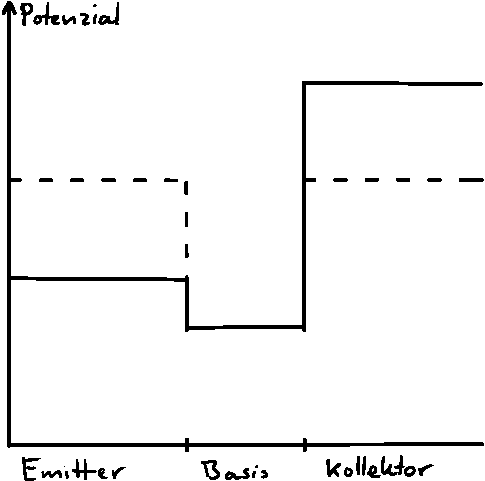
\includegraphics{Zeichnungen/B_Zeichnung.pdf}
	\caption{%
		Potenzialverlauf im npn-Transistor
	}
	\label{fig:B_Zeichnung}
\end{figure}

\FloatBarrier
\subsection{Aufgabe C}

\begin{problem}
	Wie sehen die Ladungsträgerkonzentrationen für Löcher und Elektronen im
	npn-Transistor aus?
\end{problem}

Die Ladungsträgerkonzentration im npn-Transistor ist in
Abbildung~\ref{fig:C_Zeichnung} zu sehen.

\begin{figure}
	\centering
	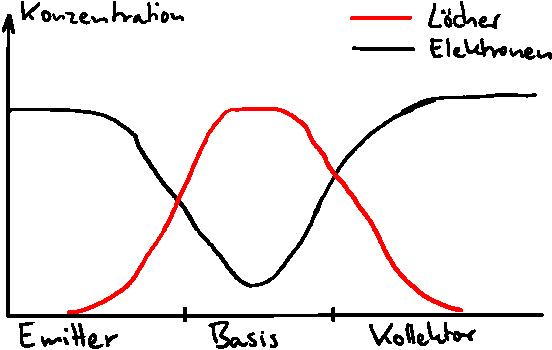
\includegraphics{Zeichnungen/C_Zeichnung.pdf}
	\caption{%
		Ladungsträgerkonzentration im npn-Transistor
	}
	\label{fig:C_Zeichnung}
\end{figure}

\FloatBarrier
\subsection{Aufgabe D}

\begin{problem}
	Verifizieren Sie die Relationen zwischen $\alpha$, $\beta$ und $\gamma$.
\end{problem}

Zwischen $\alpha$ und $\beta$:

\begin{align*}
	\beta &= \dod{\IC}{\IB}\\
	&= \dod{\IC}{\del{\IE-\IC}}\\
	&= \frac{\dif\IC}{\dif\IE-\dif\IC}\\
	&= \frac{\od\IC\IE}{\od\IE\IE-\od\IC\IE}\\
	&=\frac{\alpha}{1-\alpha}
	\intertext{Zwischen $\beta$ und $\gamma$:}
	\beta &= \dod{\IC}{\IB}\\
	&=\dod{\del{\IE-\IB}}\IB\\
	&= \frac{\dif\IE-\dif\IB}{\dif\IB}\
	&= \gamma-1
\end{align*}

\FloatBarrier
\subsection{Aufgabe E}

\begin{problem}
	Welchen Ausgangsspannunsbereich ($U_\text{out min}, U_\text{out max}$)
	(Aussteuerbereich) hat die Schaltung in Abbildung~\ref{fig:3_4-5}?
	Vernachlässigen Sie hier $U_\text{CE sat}$.
\end{problem}

\begin{figure}[htbp]
	\centering
	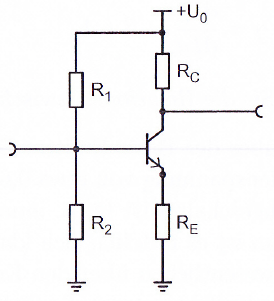
\includegraphics[width=.4\textwidth]{Anleitung/3_4-5.png}
	\caption{%
		\cite[Abbildung~3/4.5]{physik313-Anleitung}
	}
	\label{fig:3_4-5}
\end{figure}

\fehlt

\FloatBarrier
\subsection{Aufgabe F}

\begin{problem}
	Welche Form hat die \emph{Eingangskennlinie} eines Transistors in
	Emitterschaltung ($\IB$ als Funktion von $\UBE$)?
\end{problem}

Die Eingangskennlinie ist die Kennlinie einer Diode. Sie ist in
Abbildung~\ref{fig:F_Zeichnung} zu sehen.

\begin{figure}[htbp]
	\centering
	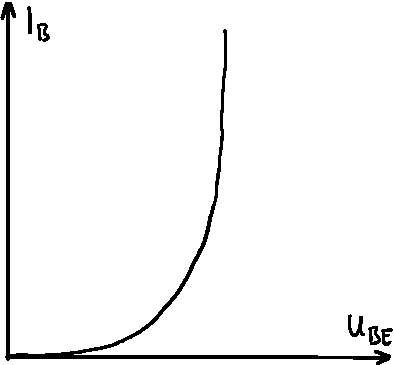
\includegraphics{Zeichnungen/F_Zeichnung.pdf}
	\caption{%
		Einganskennlinie eines Transistors in Emitterschaltung
	}
	\label{fig:F_Zeichnung}
\end{figure}

\FloatBarrier
\subsection{Aufgabe G}

\begin{problem}
	Leiten Sie \eqref{eq:3_4-7} her!
\end{problem}

Die zitierte Gleichung ist:
\begin{equation}
	\label{eq:3_4-7}
	\UB = U_0\frac{R_2}{R_1 + R_2} - \IB\frac{R_1 R_2}{R_1 + R_2}
\end{equation}

$\UB$ und $\IB$ sind in Abbildung~\ref{fig:3_4-5} die Spannung, die über $R_2$
abfällt, bzw. der Strom der durch $R_2$ fließt. $U_1$ fällt über $R_1$ ab und
der Strom $I_1$ fließt durch $R_2$ hindurch.

\begin{align*}
	U_0 &= U_1 + \UB\\
		&= R_1I_1 + \UB\\
	 &= R_1 (I_2 + \IB) + \UB\\
	 &= R_1 \IB + R_1\frac{\UB}{R_2} + \UB\\
	 &= \UB \frac{R_1+R_2}{R_2} + R_1 \IB
	\intertext{hieraus folgt sofort}
	\UB &= U_0\frac{R_2}{R_1 + R_2} - \IB\frac{R_1 R_2}{R_1 + R_2}
\end{align*}

\FloatBarrier
\subsection{Aufgabe H}

\begin{problem}
	Was passiert, wenn man den Spannungsteiler zu niederohmig macht?
\end{problem}

Wenn der Spannungsteiler zu niederohmig ist, können große Ströme durch ihn
fließen. Wenn die Betriebsspannung als ideale Spannungsquelle angenommen wird,
ändert dies nichts an der Betriebsspannung. Jedoch wird so Basis und Emitter
mit einer zu hohen Admittanz verbunden, das Eingangssignal wird geschwächt. Im
extremen Fall liegt am Transistor gar kein Signal mehr an, die Verstärkung
funktioniert nicht mehr.

\FloatBarrier
\subsection{Aufgabe I}

\begin{problem}
	Wie sieht die entsprechende Kennlinie beim bipolaren Transistor aus?
	Welcher Spannung entspricht dort $U_\text{thr}$?
\end{problem}

Die „entsprechende Kennlinie“ ist der Graph von $\ID$ gegen $\UGS$. Bei einem
bipolaren Transistor ist dies $\IC$ gegen $\UBE$.

Die Kennlinie sieht genauso aus, wie die einer normalen Diode, da Basis und
Emitter eine normale Diode sind. Die Kennlinie ist in
Abbildung~\ref{fig:beuth-bild-16-9} gezeigt.

\begin{figure}[htbp]
	\centering
	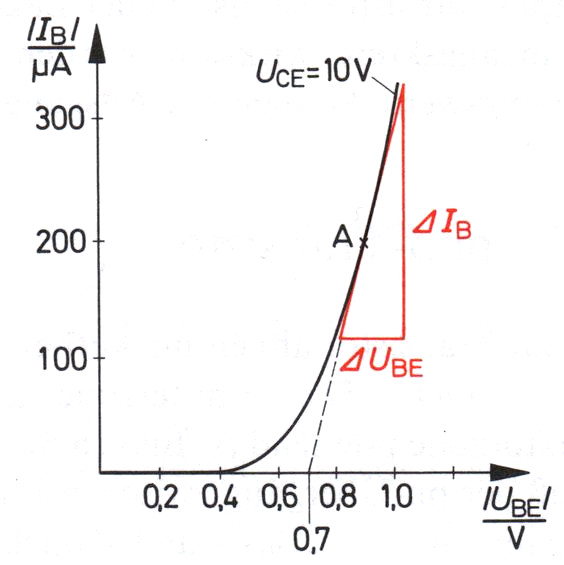
\includegraphics[width=.5\textwidth]{beuth-bild-16-9.jpg}
	\caption{%
		\cite[Bild~16.9]{beuth/elementare_elektronik}
	}
	\label{fig:beuth-bild-16-9}
\end{figure}

Die Spannung $U_\text{thr}$ entspricht hier der Spannung, die die Diode
braucht, bis sie leitend wird, also $\SI{.6}\volt$.

\FloatBarrier
\subsection{Aufgabe J}

\begin{problem}
	Was ändert sich, wenn man $\IS$ anstelle von $\ID$ aufträgt?
\end{problem}

Da $I_\text{G}\approx0$, ändert sich nichts signifikant.

\FloatBarrier
\subsection{Aufgabe K}

\begin{problem}
	Zeigen Sie, dass genauer gilt:
	\begin{equation}
		\label{eq:3_4-11}
		v = \frac{\gamma \RE}{r_\text{BE} + \gamma \RE},
	\end{equation}
	wobei der differentielle Widerstand der Emitter-Basis-Diode $r_\text{BE} =
	\dif  \UBE / \dif  \IB$ ist.
\end{problem}

Aus

\begin{align*}
	\UB &= \UBE + \UE
	\intertext{folgt}
	v &= \dod\UE\UB\\
	&= \frac{\dif\UE}{\dif\UBE+\dif\UE}\\
	&= \frac{\dif\IE\RE}{\dif\UBE+\dif\IE\RE}\\
	&= \frac{\od\IE\IB\RE}{\od\UBE\IB+\od\IE\IB\RE}\\
	&= \frac{\gamma\RE}{r_\text{BE}+\gamma\RE}
\end{align*}

\FloatBarrier
\subsection{Aufgabe L}

\begin{problem}
	Welchen Zweck könnte der Kollektorwiderstand $\RC$ beim Emitterfolger
	haben? Hinweis: Am Ausgang könnte eine niederohmige Last angeschlossen
	sein.
\end{problem}

Angenommen, laut Hinweis, dass der die Last, $\RE$ niederohmig ist. Der
Transistor wird bei großen Basisströmen auch niederohmig. Wenn dann kein
Schutzwiderstand $\RC$ vorgeschaltet ist, fließt ein hoher Strom durch die
Last.

\FloatBarrier
\subsection{Aufgabe M}

\begin{problem}
	Beweisen Sie \eqref{eq:3_4-12}.
\end{problem}

Die zitierte Gleichung ist:
\begin{equation}
	\label{eq:3_4-12}
	\frac{r_\text{out}}{r_\text{in}}
	= \frac{\gamma \RE}{r_\text{BE} + \gamma \RE}
	\approx \frac 1\gamma
\end{equation}

Aus $r_\text{in}=\frac\UB\IB$ und $r_\text{out}=\frac\UE\IE$ folgt:

\begin{align*}
	\frac{r_\text{out}}{r_\text{in}} &= \dod\UE\IE \dod\IB\UB\\
	&= \frac{\gamma\RE}{r_\text{BE}+\gamma\RE}\frac1\gamma\\
	&= \frac{\RE}{r_\text{BE}+\gamma\RE}\\
	&\approx \frac 1\gamma
\end{align*}

\FloatBarrier
\subsection{Aufgabe N}

\begin{problem}
	Wie groß ist der Eingangswiderstand des unbelasteten Emitterfolgers?
\end{problem}

\begin{align*}
	R_\text{in} &= \dod\UB\IB\\
	&= \frac {\dif\UE+\dif\UBE}{\dif\IB}\\
	&= r_\text{BE} + \dod \IE\IB \RE\\
	&= r_\text{BE} + \gamma\RE
\end{align*}

\FloatBarrier
\subsection{Aufgabe O}

\begin{problem}
	Zeigen Sie, dass genauer gilt:
	\begin{equation}
		\label{eq:3_4-14}
		v = - \frac{\beta \RC}{r_\text{BE} + \gamma \RE}
	\end{equation}
\end{problem}

\begin{align*}
	v &= \dod \UC\UB\\
	  &= -\frac{\dif\IC\RC}{\dif\UBE + \dif\UE}\\
	  &= -\frac{\dif\IC\RC}{\dif\UBE + \dif\IE\RE}\\
	  &= -\frac{\od\IC\IB\RC}{\od\UBE\IB+\od\IE\IB\RE}\\
	  &= -\frac{\beta\RC}{r_\text{BE}+\gamma\RE}
\end{align*}

\FloatBarrier
\subsection{Aufgabe P}

\begin{problem}
	Beweisen Sie \eqref{eq:3_4-17}.
\end{problem}

Die zitierte Gleichung ist:
\begin{equation}
	\label{eq:3_4-17}
	\frac{\dif  v} v
	= \frac{\dif  v_0}{v_0} \frac{1}{k v_0 + 1}
	= \frac{\dif  v_0}{v_0} \frac{v}{v_0}
\end{equation}

Aus 

\begin{align*}
	\frac 1v &= \frac 1{v_0} + k
	\intertext{folgt:}
	v &= \frac {v_0}{1+kv_0}
	\intertext{Daraus ergibt sich}
	\dod {v}{v_0} &= \frac {1+kv_0-kv_0}{\del{1+kv_0}^2}\\
	&= \frac 1{\del{1+kv_0}^2}\\
	&= \frac {v_0}{1+kv_0} \frac 1{v_0\del{1+kv_0}}\\
	&= \frac v{v_0} \frac 1{1+kv_0}
	\intertext{Hieraus erhält man die gesuchte Gleichung}
	\frac {\dif v}v &= \frac {\dif v_0}{v_0} \frac 1{1+kv_0} = \frac {\dif
v_0}{v_0} \frac v{v_0}
\end{align*}

\FloatBarrier
\subsection{Aufgabe Q}

\begin{problem}
	Erklären sie, wieso die Kapazität $C_\text{CB}$ Einfluss auf die
	Verstärkung hat.
\end{problem}

\fehlt

\FloatBarrier
\subsection{Aufgabe R}

\begin{problem}
	Erklären Sie die Funktionsweise der Schaltung in
	Abbildung~\ref{fig:3_4-15}! Wie groß ist die Spannungsänderung im Punkt P
	bei einer Stromänderung $\dif  \IE(T2)$ und welche
	Transistorgröße bestimmt diesen Wert?
\end{problem}

\begin{figure}[htbp]
	\centering
	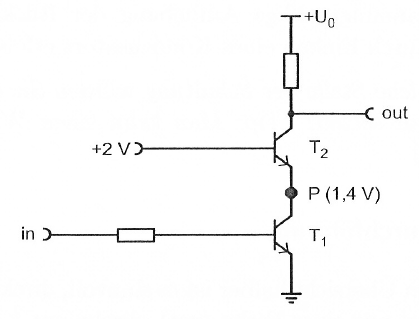
\includegraphics[width=.6\textwidth]{Anleitung/3_4-15.png}
	\caption{%
		\cite[Abbildung~3/4.15]{physik313-Anleitung}
	}
	\label{fig:3_4-15}
\end{figure}

\fehlt

\FloatBarrier
\subsection{Aufgabe S}

\begin{problem}
	Leiten Sie \eqref{eq:3_4-18} her. Hinweise: Da die Gegenkopplung bei
	Betrachtung im Frequenzraum auf der Addition von Sinusschwingungen beruht
	und wie in diesem Kapitel die Phasen ignoriert haben, ist hier
	$v(f_\text{grenz gk}) = 2v(f=0)$ statt korrekterweise $\sqrt 2 v (f = 0)$.
\end{problem}

Die zitierte Gleichung ist:
\begin{equation}
	\label{eq:3_4-18}
	f_\text{grenz gk} = f_\text{grenz} \frac{v_0}{v(f=0)}
\end{equation}

\fehlt

\FloatBarrier
\subsection{Aufgabe T}

\begin{problem}
	Erläutern Sie die Wirkungsweise der Art der Stabilisierung des
	Basispotentials durch den Widerstand $R$ in Abbildung~\ref{fig:3_4-16}.
	Überlegen Sie dazu, was passiert, wenn das Basispotential aus irgend einem
	(äußeren) Grund „wegläuft“!
\end{problem}

\begin{figure}[htbp]
	\centering
	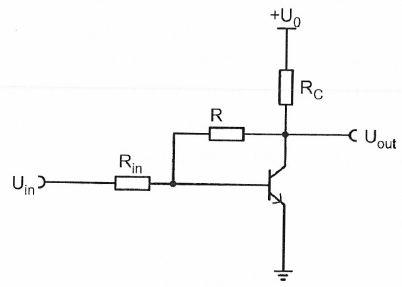
\includegraphics[width=.6\textwidth]{Anleitung/3_4-16.png}
	\caption{%
		\cite[Abbildung~3/4.16]{physik313-Anleitung}
	}
	\label{fig:3_4-16}
\end{figure}

\fehlt

%%%%%%%%%%%%%%%%%%%%%%%%%%%%%%%%%%%%%%%%%%%%%%%%%%%%%%%%%%%%%%%%%%%%%%%%%%%%%%%
%                   Durchführung: Transistoreigenschaften                    %
%%%%%%%%%%%%%%%%%%%%%%%%%%%%%%%%%%%%%%%%%%%%%%%%%%%%%%%%%%%%%%%%%%%%%%%%%%%%%%%

\FloatBarrier
\section{Durchführung Tag 1: Transistoreigenschaften}

\FloatBarrier
\subsection{Kennlinien und Arbeitspunkt}

\subsubsection{Kennlinienschreiber}

Um direkt mehrere Kennlinien auf dem Oszilloskop darstellen zu können, müssen
wir schnell hintereinander verschiedene Basisströme $\IB$ auf den Transistor
gegeben werden. Diese Umschaltung der Basisströme übernimmt der
Kennlinienschreiber für uns. Das Schaltbild des Kennlinienschreibers ist in
Abbildung~\ref{fig:3-1} dargestellt.

\begin{figure}[htbp]
	\centering
	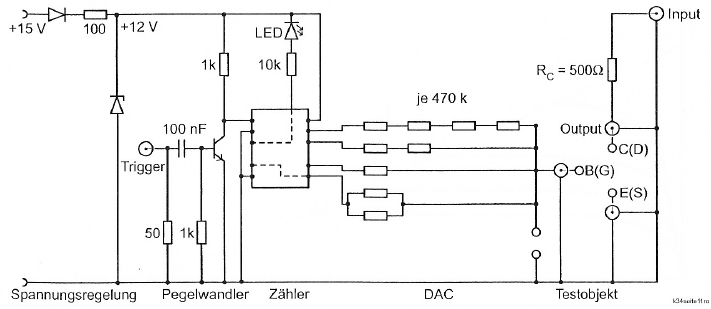
\includegraphics[width=\textwidth]{Anleitung/3-1.png}
	\caption{
		Kennlinienschreiber \cite[Abbildung~3.1]{physik313-Anleitung}
	}
	\label{fig:3-1}
\end{figure}

Am linken Triggereingang wird ein
Rechtecksignal zugeführt. Dieses wird durch den Kondensator differenziert. Die
positiven Pulse, die durch den Transistor verstärkt werden, werden im Zählwerk
gezählt. Dieses gibt die aktuelle Anzahl als vier Binärstellen durch vier
Widerstandsketten. Die einzelnen Widerstände unterscheiden sich um einen Faktor
2, so dass der Ausgangsstrom in 16 Stufen erhöht wird.

\subsubsection{Inbetriebnahme des Kennlinienschreibers}

Am rechten Ende ist ein Steckplatz für einen Transistor, der mit den oben
beschriebene den Basisströmen versorgt wird. Der zweite Ausgang des
Funktionsgenerators, der ein Dreiecksignal liefert, gibt eine kontinuierlich
ändernde Betriebsspannung. Mit dem Oszilloskop nehmen wir die
Kollektor-Emitter-Spannung $\UCE$ ab und geben es in Kanal~2 rein. Auf Kanal~1
wird die Betriebsspannung vom Funktionsgenerator angelegt. Dieser Aufbau ist in
Abbildung~\ref{fig:3-2} gezeigt.

\begin{figure}[htbp]
	\centering
	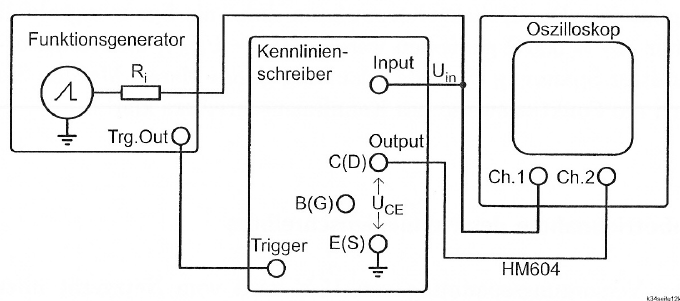
\includegraphics[width=\textwidth]{Anleitung/3-2.png}
	\caption{
		\cite[Abbildung~3.2]{physik313-Anleitung}
	}
	\label{fig:3-2}
\end{figure}

Damit auf dem Oszilloskop die Spannungsdifferenz angezeigt wird, invertieren
wir Kanal~2 und addieren ihn auf Kanal~1. Für die Kennlinien stellen wir
außerdem den XY-Betrieb ein.

Wir schließen den Transistor vom \emph{Schaltbrett~1} (siehe
Abbildung~\ref{fig:3-4}) an den Kennlinienschreiber an.

\begin{figure}[htbp]
	\centering
	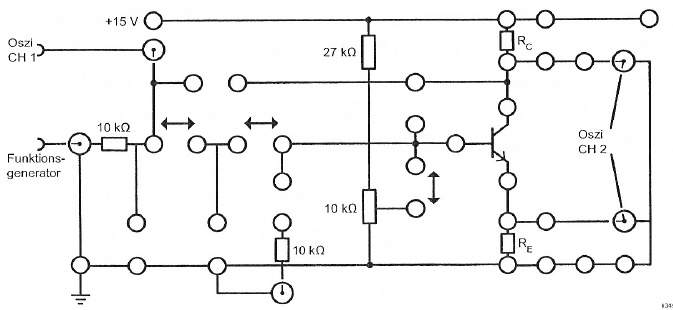
\includegraphics[width=\textwidth]{Anleitung/3-4.png}
	\caption{
		\emph{Schaltbrett~1} \cite[Abbildung~3.4]{physik313-Anleitung}
	}
	\label{fig:3-4}
\end{figure}

\subsubsection{Bipolarer Transistor}

\paragraph{Aufnahme der Kennlinen}

Wir lassen die Schaltung von unserem Assistenten überprüfen. Danach schalten
wir das Netzgerät ein und erhalten nach Justierung das Kennlinienfeld, siehe
Abbildung~\ref{fig:refactor_Kennlinienfeld}.

Den Kollektorstrom $\IC$ haben wir indirekt gemessen, in dem wir die
Spannungsdifferenz vor und nach dem Widerstand $\RC$ mit dem Oszilloskop
sichtbar gemacht haben. Da $\RC = \SI{500}\ohm$ ist, können wir die Spannung so
in einen Strom umwandeln.

\paragraph{Bestimmung von $\beta$}

Aus dem Graph in Abbildung~\ref{fig:refactor_Kennlinienfeld} lesen den Abstand
zwischen zwei Kennlinien, $\dif\IC$, ab. Wir wählen Kennline $\messwert$ und
$\messwert$, und erhalten eine Differenz von \SI{<< dIC >>}{\micro\ampere}. Mit
$\dif\IB = \SI{<< dIB >>}{\ampere}$ erhalten wir:
\[
	\beta = \dod\IC\IB = \num{<< beta >>}
\]

Die Nummer unseres \emph{Schaltbrett~1} ist: $\messwert$

\paragraph{Arbeitspunkt}

Die Arbeitsgerade ist in der Anleitung gegeben als:
\cite[Formel~3/4.6]{physik313-Anleitung}
\begin{equation}
	\label{eq:3_4-6}
	\IC = \frac{U_0 - \UCE}{\RC + \RE}
\end{equation}

Mit $\RC = \RE = \SI{390}\ohm$ und einer Betriebspannung von $U_0 =
\SI{15}\volt$ können wir eine Gerade einzeichnen. Die Spurpunkte sind:
\[
	\del{\UCE = \SI0\volt; \IC = \frac{U_0}{\RC + \RE} = \SI{19.2}{\milli\ampere}}
	\eqnsep
	\del{\UCE = U_0 = \SI{15}\volt; \IC = \SI0\ampere}
\]

Aus diesem Grund sollten wir bereits beim Abzeichnen des Kennlinienfeldes
darauf achten, dass $\UCE$ einen Bereich bis $\SI{15}\volt$ und $\IC$ einen
Bereich bis $\SI{20}{\milli\ampere}$ umfasst.

Wir zeichnen diese Gerade in den Graph in Abbildung
\ref{fig:refactor_Kennlinienfeld_Gerade} ein.

In der Anleitung war gegeben, dass die Kennlinien $(\SI{12}\volt -
\SI{.7}\volt)/(4 \cdot \SI{470}{\kilo\ohm})$, also \SI{6.01}{\micro\ampere}
auseinander liegen. Es soll die Spannung $\UCE$ für den Arbeitspunkt $\IB =
\SI{60}{\micro\ampere}$ abgeschätzt werden, in dem die Linien im Kennlinienfeld
verlängert werden. Die gewünschte Linie ist dann die zehnte Linie. Aus dem
erweiterten Kennlinienfeld in
Abbildung~\ref{fig:refactor_Kennlinienfeld_erweitert} lesen wir die Spannung
$\UCE$ ab: $\messwert$.

\subsubsection{FET}

\paragraph{Aufnahme der Kennlinien}

Wir benutzen den gleichen Aufbau, wie in der vorherigen Aufgabe. Den bipolaren
Transistor ersetzen wir durch einen FET. Da dieser mit einer Spannung gesteuert
wird, müssen wir den Basisstrom $\IB$ erst noch in eine Basis-Emitter-Spannung
$\UBE$ umwandeln. Bei FETs heißt diese jedoch Gate-Source-Spannung, $\UGS$. Wir
schließen also einen Widerstand $R$ zwischen Gate und Source an. Dazu benutzen
wir ein \SI{470}{\kilo\ohm}-Potentiometer. Wir justieren das Potentiometer so,
dass möglichst viele Linien auf dem Oszilloskop zu sehen sind.

Den Spannungsabstand $\dif\UGS$ erhalten wir durch $R \cdot
\SI{6}{\micro\ampere}$, da, wie schon im vorherigen Abschnitt berechnet, die
Stromunterschiede $\dif\IB$ den Wert \SI{6}{\micro\ampere} haben. Über einem
Widerstand $R$ fällt dann die Spannung $U = IR$ ab. Dies ist natürlich nicht
ganz exakt, da der Widerstand nicht unendlich groß ist und so alle Ströme etwas
verändert.

\paragraph{Bestimmung der Schwellenspannung und Transkonduktanz}
\label{par:Schwellenspannung}

\fehlt

\FloatBarrier
\subsection{Emitterfolger}

\subsubsection{Aufbau}

Auf dem \emph{Schaltbrett~1} (Abbildung~\ref{fig:3-4}) bauen wir einen
Emitterfolger (Kollektorschaltung) auf. Eine solche ist, mit Kapazitäten
erweitert, in Abbildung~\ref{fig:beuth-bild-16-21} dargestellt.

\begin{figure}[htbp]
	\centering
	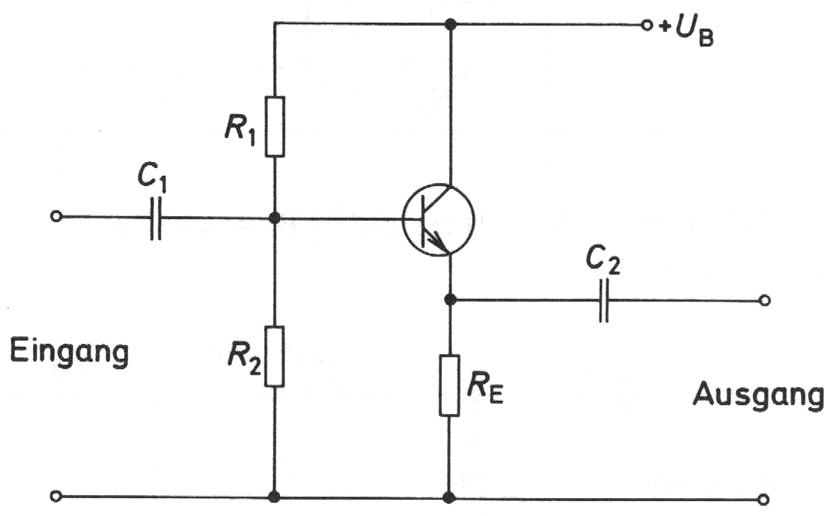
\includegraphics[width=.6\textwidth]{beuth-bild-16-21.jpg}
	\caption{%
		Verstärkerstufe in Kollektorschaltung (Emitterfolgerstufe)
		\cite[Bild~16.21]{beuth/elementare_elektronik}
	}
	\label{fig:beuth-bild-16-21}
\end{figure}

Das Netzgerät mit $U_0 = \SI{15}\volt$ wird an das Schaltbrett angeschlossen.
Wir setzen $\RC = \RE = \SI{390}\ohm$ ein, wie in der Anleitung beschrieben.
Als Signal stellen wir ein Sinussignal mit $\dif\UBE = \SI{.5}{\voltss}$ und
einer Frequenz $f = \SI{500}\hertz$ ein. Dazu kommt ein Offset von
\SI{2}{\volt}.

Das Oszilloskop wir mit Kanal~1 an das Signal des Funktionsgenerators
angeschlossen. Kanal~2 kommt Emitter und Emitterwiderstand $\RE$, da es sich um
eine Kollektorschaltung handelt.

Wir vergleichen die Eingangs- und Ausgangsspannung, $\UB$ bzw. $\UE$. auf dem
Oszilloskop.

\textcolor{gray}{
	(Dies habe ich mir nur überlegt, sollte durch die Messung ersetzt werden.)
	Eingangs- und Ausgangspannung haben die gleiche Phase. Das liegt daran,
	dass ein höherer Basisstrom $\IB$ einen höheren Kollektorstrom $\IC$
	erlaubt, da weniger Spannung $\UCE$ abfällt. Dies führt dazu, dass mehr
	Strom durch den Emitterwiderstand $\RE$ fließt und somit mehr Spannung
	$\UE$ abfällt.
}

\subsubsection{Spannungsverstärkung}

Wir messen die Spannungsverstärkung $\dif\UE/\dif\UB$. Dazu lesen wir vom
Oszilloskop die Spitze-Spitze-Spannung von beiden Kanälen ab und erhalten:
\[
	\dif\UE = \SI{<< dU_E >>}\voltss
	\eqnsep
	\dif\UB = \SI{<< dU_B >>}\voltss
\]

Daraus folgt die Spannungsverstärkung $\dif\UE/\dif\UB = \num{<<
spannungsverstaerkung >>}$.

\subsubsection{Aussteuergrenzen}

\fehlt

\subsubsection{Arbeitspunkteinstellung}

Wir ersetzen nun den DC-Offset am Funktionsgenerator mit einer
Basisvorspannung, die wir mit dem Spannungsteiler erzeugen. In der Anleitung
steht: „Fügen Sie dazu einen geeigneten Kondensator in Serie hinter dem
\SI{10}{\kilo\ohm}-Widerstand ein.“ Auf \emph{Schaltbrett~1} gibt es jedoch
drei solche Widerstände, wobei einer davon ein Potentiometer ist. Der
Kondensator soll hinter den linken Widerstand. Dies habe ich in blau in
Abbildung~\ref{fig:3-4_Arbeitspunkt} dargestellt. In rot und grün sind
einfache Kabelbrücken.

\begin{figure}[htbp]
	\centering
	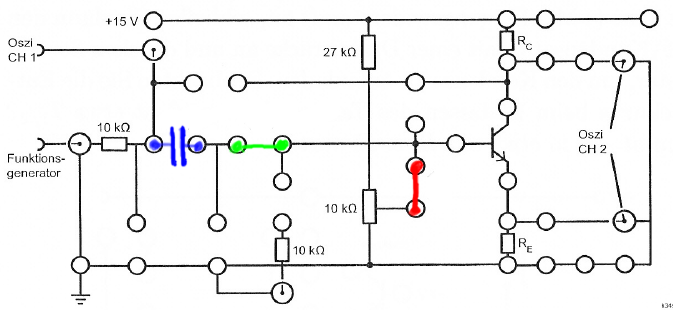
\includegraphics[width=\textwidth]{Anleitung/3-4_Arbeitspunkt.png}
	\caption{
		\emph{Schaltbrett~2} mit Beschaltung. Originalbild ist in
		Abbildung~\ref{fig:3-4} und aus
		\cite[Abbildung~3.4]{physik313-Anleitung}.
	}
	\label{fig:3-4_Arbeitspunkt}
\end{figure}

Der Kondensator hat nicht direkt etwas mit der Einstellung der Basisvorspannung
zu tun. Diese ist mit dem roten Kontakt schon eingestellt. Der Kondensator
dient dazu, den Funktionsgenerator von der Gleichspannung zu entkoppeln, sowie
eine eventuell verbleibende Offsetspannung vom Signal zu trennen.

Wenn der Kondensator zu klein ist, ist seine Impedanz zu hoch, das
Eingangssignal wird geschwächt.

\textcolor{gray}{
	Die Eigenschaften der Schaltung sollten jetzt etwas anders sein, weil der
	Kondensator das Eingangssignal differenziert. Bei einer Sinusspannung
	bedeutet das nur eine Phasenverschiebung um $\piup/2$. Somit sind die
	beiden Signale auf den Kanälen des Oszilloskops im Vergleich zu vorher
	miteinander verschoben.
}

Wir verändern den Spannungsteiler um zu schauen, wann der Aussteuerungsbereich
der Schaltung am größten ist.

\fehlt

\FloatBarrier
\subsection{FET}

Auf dem \emph{Schaltbrett~2} (Abbildung~\ref{fig:3-5}) bauen wir eine
Emitterfolgerschaltung (Kollektorschaltung) mit dem Bipolartransistor auf.
Dabei setzen wir $\RC = \SI0\ohm$ und den Emitterwiderstand im Bereich
\SIrange{1}{2}{\kilo\ohm}.

\FRAGE{
	Im Schaltbild ist ein \SI{100}{\ohm}-Widerstand eingezeichnet. Wo soll der
	zusätzliche Widerstand hin, mit dem dann in den \si{\kilo\ohm}-Bereich
	gegangen wird?
}

Die Schaltung wird mit \SI{10}{\volt} Gleichstrom versorgt. Als Eingangssignal
in die Basis des Transistors geben wir ein Sinussignal mit \SI1{\kilo\hertz}
und \SI{2}{\voltss}. Außerdem stellen wir einen Offset von etwa \SI5{\volt}
ein.

\begin{figure}[htbp]
	\centering
	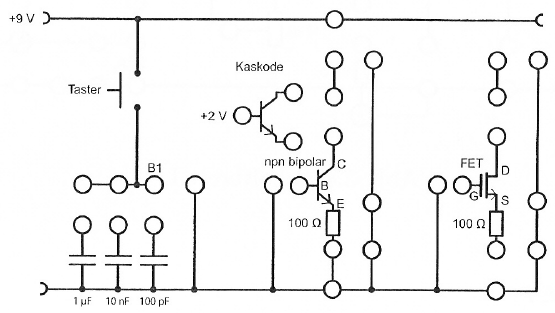
\includegraphics[width=\textwidth]{Anleitung/3-5.png}
	\caption{
		\emph{Schaltbrett~2} \cite[Abbildung~3.5]{physik313-Anleitung}
	}
	\label{fig:3-5}
\end{figure}

Wir beobachen das Eingangssignal sowie das Signal, das aus dem Emitter kommt,
mit den beiden Kanälen des Oszilloskops. Dazu stellen wir auf beiden Kanälen
die gleiche Verstärkung und den gleichen $y$-Offset ein. Die Kanäle werden auf
DC gekoppelt, damit auch die Basisvorspannung zu sehen ist.

Der Offset wird varriert, dabei beobachten wir \fehlt.

Als nächstes bauen wir eine vergleichbare Schaltung, diesmal allerdings mit dem
FET. Die Schaltung heißt nicht mehr Emitterfolgerschaltung sondern
Sourcefolgerschaltung, da beim FET die englischen Begriffe benutzt werden. Wir
überprüfen die Funktion der Schaltung und verändern den DC-Offset und
beobachten \fehlt.

Wir bestimmen $U_\text{thr}$ zu $\messwert$. Im Vergleich zu der Messung der
Schwellenspannung, die wir auf Seite \pageref{par:Schwellenspannung} gemessen
haben, \fehlt

\subsubsection{Eingangswiderstand}

In dieser Versuchsaufgabe wollen wir die Eingangswiderstände der Transistoren
als unbelastete Emitterfolger abschätzen.

Den Sinusgenerator nehmen wir aus der Buchse~B1 heraus. Mit einer Drahtbrücke
koppeln wir den \SI1{\micro\farad}-Kondensator ein. Das Oszilloskop hat einen
Eingangswiderstand von \SI1{\mega\ohm}. Dadurch sollte die Zeitkonstante für
die Entladung des Kondensators sein:
\[
	\tau = RC = \SI1{\second}
\]

Die Halbwertszeit $T_{1/2}$ ist um $1/\ln(2)$ kleiner, also $\SI{.69}\second$.
Wir beobachten eine Halbwertszeit von $\messwert$.

\TODO{
	Übereinstimmung mit Erwartung
}

Der bipolare Transistor wird wieder als Emitterfolger eingesetzt. Buchse~1 wird
mit einem kurzen BNC Kabel an die Basis angeschlossen. Mit dem Oszilloskop
beobachen wir die Spannung am Emitter, also am Ausgang des Verstärkers. Wir
beobachten die neue Abfallszeit. Diese ist anders, da der Kondensator jetzt
über einen anderen Widerstand entlädt, den Transistor. Wir beobachten eine
Abfallzeit von $\messwert$.

Aus diesem Verhältnis bestimmen wir die Stromverstärkung. Diese ist definiert
als:
\[
	B := \frac\IC\IB
	\eqnsep
	\beta := \frac{\dif\IC}{\dif\IB}
\]

\FRAGE{
	In der Anleitung werden noch weitere Stromverstärkungsgrößen, $\alpha$ und
	$\gamma$ definiert. Welche dieser Größen ist denn jetzt die Richtige?
}

\fehlt

%%%%%%%%%%%%%%%%%%%%%%%%%%%%%%%%%%%%%%%%%%%%%%%%%%%%%%%%%%%%%%%%%%%%%%%%%%%%%%%
%                    Durchführung: Transistorverstärker                     %
%%%%%%%%%%%%%%%%%%%%%%%%%%%%%%%%%%%%%%%%%%%%%%%%%%%%%%%%%%%%%%%%%%%%%%%%%%%%%%%

\FloatBarrier
\section{Durchführung Tag 2: Transistorverstärker}

\subsection{Fortsetung Emitterfolger}

\subsubsection{Spannungsverstärkung des Emitterfolgers}

\fehlt

\subsubsection{Emitterfolger als Impedanzwandler}

\fehlt

\subsection{Invertierender Transistorverstärker (Emitterschaltung)}

\subsubsection{Phasenbeziehung zwischen Ein- und Ausgang}

\fehlt

\subsubsection{Spannungsverstärkung des inverteierenden Verstärkers}

\fehlt

\subsubsection{Bestimmung des Transistoreingangswiderstands}

\fehlt

\subsection{Wechselstrommäßige Aufhebung der Gegenkopplung}

\fehlt

\subsection{Frequenzverhalten und Kaskodenschaltung}

\fehlt

\subsection{Verstärker mit Spannungsgegenkopplung}

\fehlt

\begin{figure}[htbp]
	\centering
	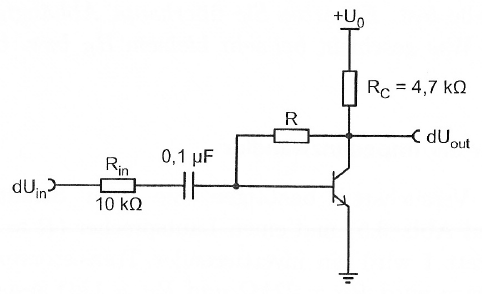
\includegraphics[width=.6\textwidth]{Anleitung/4-1.png}
	\caption{
		\cite[Abbildung~4.1]{physik313-Anleitung}
	}
	\label{fig:4-1}
\end{figure}

%%%%%%%%%%%%%%%%%%%%%%%%%%%%%%%%%%%%%%%%%%%%%%%%%%%%%%%%%%%%%%%%%%%%%%%%%%%%%%%
%                                  Literatur                                  %
%%%%%%%%%%%%%%%%%%%%%%%%%%%%%%%%%%%%%%%%%%%%%%%%%%%%%%%%%%%%%%%%%%%%%%%%%%%%%%%

\FloatBarrier
\IfFileExists{\bibliographyfile}{
	\bibliography{\bibliographyfile}
}{}

\end{document}

% vim: spell spelllang=de tw=79
